\documentclass[titlepage]{jsreport}

\usepackage[dvipdfmx]{graphicx}
\usepackage{listings}
\usepackage{cite}
\usepackage{url}
\usepackage{master_thesis}

% ソースコードを挿入するための設定
\lstset{
 	language = Python,
     frame = tbrl
}

% 修論タイトル(和文)
\title{修士論文執筆におけるLaTeXテンプレート利用の効率についての研究}

% 修論タイトル(英文)
\englishtitle{A study on the efficiency of using \LaTeX templates in writing master thesis}

% 著者名
\author{修論各代}

% 学籍番号
\studentnumber{12345678}

% 指導教員名
\advisor{指導島巣}

% 指導教員の職名
\advisortitle{准教授}

% 年度(Academic Year)
\academicyear{2021} 

% 提出年月
\submitdate{2022年3月} 

% 和文要旨
\japaneseabstract{%
象の卵はおいしいぞう。象の卵はおいしいぞう。象の卵はおいしいぞう。象の卵はおいしいぞう。象の卵はおいしいぞう。象の卵はおいしいぞう。象の卵はおいしいぞう。象の卵はおいしいぞう。象の卵はおいしいぞう。象の卵はおいしいぞう。象の卵はおいしいぞう。象の卵はおいしいぞう。象の卵はおいしいぞう。象の卵はおいしいぞう。象の卵はおいしいぞう。象の卵はおいしいぞう。象の卵はおいしいぞう。象の卵はおいしいぞう。象の卵はおいしいぞう。象の卵はおいしいぞう。象の卵はおいしいぞう。

象の卵はおいしいぞう。象の卵はおいしいぞう。象の卵はおいしいぞう。象の卵はおいしいぞう。象の卵はおいしいぞう。象の卵はおいしいぞう。象の卵はおいしいぞう。象の卵はおいしいぞう。象の卵はおいしいぞう。象の卵はおいしいぞう。象の卵はおいしいぞう。象の卵はおいしいぞう。象の卵はおいしいぞう。象の卵はおいしいぞう。象の卵はおいしいぞう。象の卵はおいしいぞう。象の卵はおいしいぞう。象の卵はおいしいぞう。象の卵はおいしいぞう。象の卵はおいしいぞう。象の卵はおいしいぞう。
}

% 英文要旨
\englishabstract{%
Elephant eggs are so delicious. Elephant eggs are so delicious. Elephant eggs are so delicious. Elephant eggs are so delicious. Elephant eggs are so delicious. Elephant eggs are so delicious. Elephant eggs are so delicious.

Elephant eggs are so delicious. Elephant eggs are so delicious. Elephant eggs are so delicious. Elephant eggs are so delicious. Elephant eggs are so delicious. Elephant eggs are so delicious. Elephant eggs are so delicious.

Elephant eggs are so delicious. Elephant eggs are so delicious. Elephant eggs are so delicious. Elephant eggs are so delicious. Elephant eggs are so delicious. Elephant eggs are so delicious. Elephant eggs are so delicious.
}

\begin{document}
\maketitle
\pagenumbering{roman}

\tableofcontents
\pagestyle{plain}
\setcounter{page}{1}

\chapter{はじめに} \label{chap:introduction}
\pagenumbering{arabic}

「はじめに」もしくは「緒言」では、研究背景、目的、そして論文の構成を書く。第一章の前に目次をつける場合、目次のページ番号はi, ii,とローマ数字にして、本文からアラビア数字にするのが一般的だ。それを実現するため、\verb|\begin{document}|の直後にページ番号をローマ数字にするコマンド\verb|\pagenumbering{roman}|が、最初の\verb|\chapter|の後にアラビア数字にするコマンド\verb|\pagenumbering{arabic}|が挿入されている。

\section{研究の背景}

研究の背景は「なぜこの研究をしなければならないか」を、「大きい理由から小さい理由」へ書いていく。「大きい理由」は、「エネルギー問題」「安全」「便利」といった、「多くの人がほぼ納得するような理由」を挙げる。次に、その「大きな理由」を実現するために、これまでどのような試みがなされてきたかを説明する。これまでに読んだ論文のイントロダクションを参考に、必要な文献を引用しながら説得力のある文章を書くこと。

\section{研究の目的}

研究の背景を受けて、この研究分野は重要であるが、なんらかの不満点があることを述べる。その不満点は解決すべき問題であることを文献を引用しながら読者に納得させる。本研究の目的は、その不満点を解消することであることを述べ、その方法について簡単に述べる。

\section{本論文の構成}

論文の構成を説明する。まず本研究の目的を一行で書いてから、各章に何が書いてあるかを説明する。以下は例である。

\begin{quotation}
    本研究では、では、分野Aにおける手法Xの精度改善を行う。以下に本論文の構成を示す。第\ref{chap:introduction}章では、分野Aにおける手法の概観を紹介し、手法Xが広く用いられていることを示した。第\ref{chap:method}章では、本研究で用いる手法X、及びその改善手法であるX'について説明する。第\ref{chap:results}章では、本研究で提案した手法X'と、もととなった手法Xとの精度の比較を行う。第\ref{chap:summary}章では本研究で得られた知見を総括し、結論と今後の展望について述べる。
\end{quotation}

\chapter{手法} \label{chap:method}

\section{引用の仕方}

原則として科学技術論文では、引用のない文章は「著者のオリジナル」であるとみなされる。LAMMPSなどのツールを使えばその関連論文を、手法の説明をするならその手法を提案した論文を引用しなければならない。

引用するのは、原則として書籍か査読論文とし、ウェブサイトの引用はさけること。特に何かの説明の参照先としてWikipediaやSlideShareなどを挙げないこと。機械学習の論文であればプレプリント(arXiv)を読むことも多いと思われるが、引用したくなるような論文はどこかのカンファレンスに採択されていることが多いので、そちらを引用すること。たとえ自分がWikipediaで知識を得たとしても、Wikipediaで引用されている文献にあたり、書籍なり論文なりを参考にすること。

参考文献は、原則としてBibTeXで管理すること。これにより、「本文で参照されていない文献を参考文献に入れてはならない」「本文で参照される順番に並べないとならない」などのルールが自動的に満たされる。

BibTeXでは、参考文献を「エントリ」と呼ばれる構造で管理する。エントリにはいくつか種別があるが、良く使うのは書籍(book)、論文(article)、プロシーディング(inproceedings)などであろう。例えば書籍は以下のようなエントリとする。

\begin{lstlisting}[language=TeX]
@book{okumura2020,
    author    = {奥村 晴彦 and 黒木 裕介},
    title     = {LaTeX2ε美文書作成入門},
    publisher = {技術評論社},
    year      = {2020}
}
\end{lstlisting}

これをTeXファイル中で以下のように引用する。

\begin{verbatim}
本論文の執筆にあたり、LaTeXの書き方については奥村・黒木の書籍を参考にした\cite{okumura2020}。
\end{verbatim}

これは以下のようにタイプセットされる。
\begin{quotation}
    本論文の執筆にあたり、LaTeXの書き方については奥村・黒木の書籍を参考にした\cite{okumura2020}。
\end{quotation}


GitHubのサイトなど、やむを得ずURLを引用する場合には、bibitemのmiscを使って以下のようにする。

\begin{lstlisting}[language=TeX]
@misc{github,
  howpublished = {\url{https://github.com/kaityo256/rbs}
},
\end{lstlisting}

例えば

\begin{verbatim}
この論文の参照実装はGitHubにて利用可能である\cite{github}。
\end{verbatim}
として引用すると、

\begin{quotation}
    この論文の参照実装はGitHubにて利用可能である\cite{github}。
\end{quotation}
となる。

\chapter{結果} \label{chap:results}

\section{図の入れ方}

図は、数が多くなければとりえあずfigといったディレクトリにまとめて入れておくと良いだろう。数が増えてきて管理が難しくなったら節ごとにわけるなど工夫すること。画像ファイルは原則としてPDFにすること。例えば\verb|temperature.pdf|を入れたいなら、

\begin{lstlisting}[language=TeX]
    \begin{figure}[htbp]
        \begin{center}
            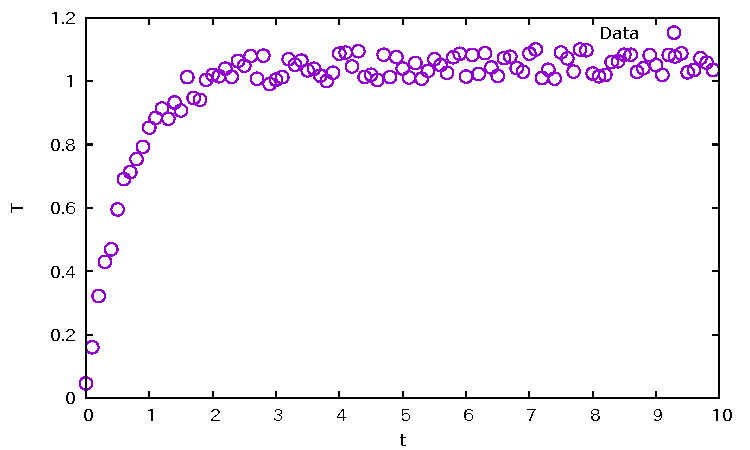
\includegraphics[width=10cm]{fig/temperature.pdf}
        \end{center}
        \caption{温度の時間発展。}
        \label{fig:temperature}
    \end{figure}
\end{lstlisting}

とすると、以下のような図が得られる。

\begin{figure}[htbp]
    \begin{center}
        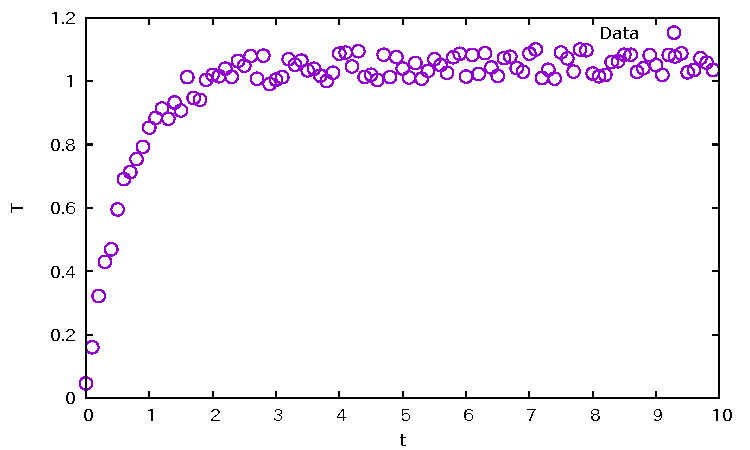
\includegraphics[width=10cm]{fig/temperature.pdf}
    \end{center}
    \caption{温度の時間発展。}
    \label{fig:temperature}
\end{figure}

この時、元データと、データからPDFを作るためのプロットファイルもしくはスクリプトファイルを一緒に入れておく。この時、画像ファイルとプロットファイルの名前を同じにしておくと良い。例えばgnuplotを使って\verb|temperature.pdf|という画像を作るなら、プロットファイルを\verb|temperature.plt|にしておく。すると、

\begin{lstlisting}[language=bash]
gnuplot temperature.plt
\end{lstlisting}

を実行することで\verb|temperature.pdf|ができるのでわかりやすい。

また、名前を揃えておくとmakefileとの相性が良くなる。例えば\verb|pressure.pdf|、\verb|temperature.pdf|、\verb|error.pdf|の三つのファイルが、同名のpltファイルから作成されるなら

\lstinputlisting[language=make]{fig/makefile}

といったmakefileを作っておけば、make一発で三つのファイルを作ることができるので便利だ。

もちろんPythonのMatplotlibを使っても良いが、いずれにせよ「データとスクリプトからコマンド一発で図のファイルが作成できる状況にしておく。

\chapter{考察および結論} \label{chap:summary}

考察は、「研究の背景」及び「目的」において提起した問題に正しく答えるようにする。得られた結果は満足すべきものだったか?不満があるならその理由はなにか?解決できそうなのか?また、「大きい理由」にも言及する。本研究によりどのような課題が見つかったかを書き、この分野における「研究の流れ」においてのような位置づけにあるかを説明した上で、今後、どのような発展の方向があるかについて書く。

\chapter*{謝辞}

謝辞は卒業論文を執筆するにあたって、お世話になった人への感謝の気持ちを書く。まず指導教員、次にお世話になった先生、研究室の助教や研究員、その他研究の相談に載ってもらったり、アドバイスをもらった人への感謝を書く。次に研究室の仲間に一言ずつ。最後に家族、特に両親への感謝で締めると良い。

\appendix

\chapter{ソースコード}

\lstinputlisting[caption = 適当なPythonスクリプト, label = prog:sample]{src/sample.py}

\bibliographystyle{junsrt}
\bibliography{reference}

\end{document}
